\section{Normalization for Time Series Forecasting} \label{related-content}

\paragraph{Global normalization.}
Standard normalization uses statistics estimated over the training data:
\begin{equation}
    \tilde{x}=\frac{x-\mu}{\sigma+\epsilon}, \qquad
    \mu=\frac{1}{N}\sum_{x\in\mathcal{D}}\frac{1}{L}\sum_{i=1}^Lx_i.
\end{equation}
It improves numerical conditioning, but the fixed statistics may cease to
describe future dates or unseen series. Related normalization layers vary the
dimensions and population used to estimate statistics; BatchNorm
\citep{batchnorm}, LayerNorm \citep{layernorm}, and GroupNorm
\citep{groupnorm} are familiar examples. In this work, we focus on input
normalization rather than hidden-layer normalization.

\paragraph{Reversible instance normalization.}
Drawing on instance normalization \citep{instancenorm}, RevIN \citep{revin}
computes statistics independently for each look-back window:
\begin{equation}
\mu_x = \frac{1}{L}\sum_{i=1}^L x_i, \qquad
\sigma_x^2 = \frac{1}{L}\sum_{i=1}^L(x_i-\mu_x)^2.
\end{equation}
For a forecaster $f_\theta$, its affine version applies
\begin{equation}
\tilde{x}=\alpha\frac{x-\mu_x}{\sigma_x+\epsilon}+\beta,
\qquad
\hat{y}=(\sigma_x+\epsilon)
\frac{f_\theta(\tilde{x})-\beta}{\alpha+\epsilon}+\mu_x.
\end{equation}
The pipeline standardizes a look-back, applies global learnable parameters
$(\alpha,\beta)$, forecasts, reverses the affine transform, and returns to data
space. \Cref{fig:revin-process} illustrates these steps.

\begin{figure}[h!]
    \centering
    \vspace{-5mm}
    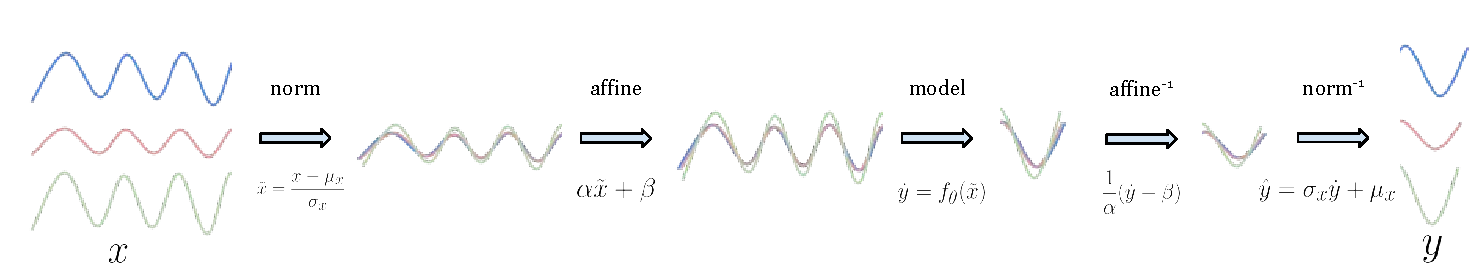
\includegraphics[width=\linewidth]{Images/min/illustrated_revin.pdf}
    \vspace{-5mm}
    \caption{Illustration of the RevIN process on three synthetic examples.}
    \label{fig:revin-process}
\end{figure}

\paragraph{The central trade-off.}
Per-window normalization guarantees zero input mean and unit input variance
before the optional affine layer. This can remove nuisance offset and scale
differences across dates and series. However, two windows that differ only in
absolute level or scale then become indistinguishable to the backbone. Instance
normalization should therefore help when those statistics vary across domains
without changing the normalized forecasting relationship, and can hurt when
they carry predictive information. Our experiments isolate this trade-off and
the separate optimization effect of weighting errors in normalized space; we
do not introduce a new normalization architecture.
